%!TEX TS-program = lualatex
%!TEX encoding   = UTF-8 Unicode

\documentclass[aspectratio=169]{beamer}

\usefonttheme{default}
\usefonttheme{professionalfonts}

\usepackage{booktabs}
\usepackage{dsfont}
\usepackage{fontspec}
\usepackage{multirow}
\usepackage{mathpazo}
\usepackage{manfnt}
\usepackage{pifont}
\usepackage{siunitx}
\usepackage{xspace}

\usepackage{appendixnumberbeamer}

\usepackage[T1]{fontenc}

\sisetup{
  detect-weight           = true,
  detect-inline-weight    = math,
  separate-uncertainty    = true,
  table-align-uncertainty = true,
  table-text-alignment    = center,
}

\defaultfontfeatures{
    Ligatures = TeX, % Ensures that dashes etc. are typeset properly
    %Numbers   = {%
    %  Monospaced,    % Always use monospaced numbers
    %  Lining         % Always use lining numbers
    %},
}

\usepackage[british]{babel}

%%%%%%%%%%%%%%%%%%%%%%%%%%%%%%%%%%%%%%%%%%%%%%%%%%%%%%%%%%%%%%%%%%%%%%%%
% Mathematics
%%%%%%%%%%%%%%%%%%%%%%%%%%%%%%%%%%%%%%%%%%%%%%%%%%%%%%%%%%%%%%%%%%%%%%%%

\usepackage{amsmath}
\usepackage{amssymb}

% Use bold font to indicate vectors
\let\vec\mathbf

\newcommand{\betti}        [1]{\ensuremath{\beta_{#1}}}
\newcommand{\diagram}         {\ensuremath{\mathcal{D}}}
\newcommand{\featurevector}[1]{\ensuremath{\mathcal{F}_{#1}}}
\newcommand{\graph}           {\ensuremath{\mathcal{G}}}
\newcommand{\landau}       [1]{\ensuremath{\mathcal{O}\left(#1\right)}}
\newcommand{\real}            {\ensuremath{\mathds{R}}}

\DeclareMathOperator{\ccount}     {\mathfrak{z}} % persistent cycle counter function
\DeclareMathOperator{\dist}       {dist}         % distance functor
\DeclareMathOperator{\flabel}     {l}            % label function
\DeclareMathOperator{\pcount}     {\mathfrak{p}} % persistent counter function
\DeclareMathOperator{\persistence}{pers}         % persistence function

\let\originalleft\left
\let\originalright\right
\renewcommand{\left}{\mathopen{}\mathclose\bgroup\originalleft}
\renewcommand{\right}{\aftergroup\egroup\originalright}

%%%%%%%%%%%%%%%%%%%%%%%%%%%%%%%%%%%%%%%%%%%%%%%%%%%%%%%%%%%%%%%%%%%%%%%%
% Plots & graphics
%%%%%%%%%%%%%%%%%%%%%%%%%%%%%%%%%%%%%%%%%%%%%%%%%%%%%%%%%%%%%%%%%%%%%%%%

\usepackage[absolute,overlay]{textpos}

\usepackage{tikz}
\usepackage{pgfplots}

\usepgfplotslibrary{external}
\usepgfplotslibrary{groupplots}

\tikzexternalize
\tikzsetexternalprefix{Figures/External/}

\pgfplotsset{compat=1.16}

\definecolor{cardinal} {RGB}{196, 30, 58}
\definecolor{lightgrey}{RGB}{230,230,230}

\pgfplotsset{%
  /pgfplots/colormap={mlcb}{rgb255=(196,30,58) rgb255=(80,200,120) rgb255=(49,140,231)}
}

%%%%%%%%%%%%%%%%%%%%%%%%%%%%%%%%%%%%%%%%%%%%%%%%%%%%%%%%%%%%%%%%%%%%%%%%
% Theming
%%%%%%%%%%%%%%%%%%%%%%%%%%%%%%%%%%%%%%%%%%%%%%%%%%%%%%%%%%%%%%%%%%%%%%%%

\setsansfont{Myriad Pro}
\setmonofont{Hack}

\setbeamercolor{alerted text}           {fg=cardinal      }
\setbeamercolor{bibliography entry note}{fg=black         }
\setbeamercolor{structure}              {fg=black,bg=white}
\setbeamercolor{normal text}            {fg=black,bg=white}
\setbeamercolor{frametitle}             {fg=black,bg=white}
\setbeamercolor{item projected}         {fg=black,bg=white}
\setbeamercolor{footline colour}        {fg=black,bg=white}

\setbeamertemplate{caption}                         {\insertcaption}
\setbeamertemplate{itemize items}[circle]

% Workaround for text bullets that are too large. I do not know their
% root cause.
\setbeamertemplate{itemize items}{%
  \textbullet
}

\setbeamertemplate{enumerate items}   [square]
\setbeamertemplate{navigation symbols}              {}

%\setbeamerfont{title}     {family=\fontspec{Libre Franklin Bold}}
%\setbeamerfont{frametitle}{family=\fontspec{Libre Franklin Bold}}
%\setbeamerfont{author}    {family=\fontspec{Libre Franklin Bold}}

\setbeamertemplate{footline}{%
  \leavevmode%
  \hbox{%
    \begin{beamercolorbox}[wd=.075\paperwidth, ht=2.5ex, dp=2ex, left]{footline colour}%
      \hspace*{2.5mm}\includegraphics[height=1.5ex]{Figures/Logo_D-BSSE}%
    \end{beamercolorbox}%
    \begin{beamercolorbox}[wd=.925\paperwidth, ht=2.5ex, dp=2ex, right]{footline colour}%
      \usebeamerfont{title in head/foot}\insertshorttitle%
      \hspace*{3.14mm}%
      \hspace*{3.14mm}\insertdate%
      \hspace*{4.5mm}%
    \end{beamercolorbox}%
  }
}

% Disable rules for footnotes; this makes the display less cluttered in my opinion.
\renewcommand{\footnoterule}{}

\makeatletter
\addtobeamertemplate{block begin}{
\def\@listi{\leftmargin\leftmargini
              \topsep    0pt
              \parsep    0pt
              \itemsep   3pt plus 2pt minus 3pt}
\partopsep 0pt
}
\makeatother

\AtBeginSection[]
{
  \begin{frame}<beamer>
    \frametitle{Outline}
    \tableofcontents[currentsection]
  \end{frame}
}

%%%%%%%%%%%%%%%%%%%%%%%%%%%%%%%%%%%%%%%%%%%%%%%%%%%%%%%%%%%%%%%%%%%%%%%%
% Algorithms
%%%%%%%%%%%%%%%%%%%%%%%%%%%%%%%%%%%%%%%%%%%%%%%%%%%%%%%%%%%%%%%%%%%%%%%%

\usepackage{algorithm}
\usepackage{algorithmicx}
\usepackage{algpseudocode}

%%%%%%%%%%%%%%%%%%%%%%%%%%%%%%%%%%%%%%%%%%%%%%%%%%%%%%%%%%%%%%%%%%%%%%%%
% Typography
%%%%%%%%%%%%%%%%%%%%%%%%%%%%%%%%%%%%%%%%%%%%%%%%%%%%%%%%%%%%%%%%%%%%%%%%

\renewcommand{\th}{\textsuperscript{\textup{th}}\xspace}

\newcommand{\yes}{\textcolor{eth-4}{\ding{51}}}
\newcommand{\no} {\textcolor{eth-7}{\ding{55}}}

%%%%%%%%%%%%%%%%%%%%%%%%%%%%%%%%%%%%%%%%%%%%%%%%%%%%%%%%%%%%%%%%%%%%%%%%
% Title
%%%%%%%%%%%%%%%%%%%%%%%%%%%%%%%%%%%%%%%%%%%%%%%%%%%%%%%%%%%%%%%%%%%%%%%%

\title{Machine Learning for Biology}
\date{28 June 2019}

%%%%%%%%%%%%%%%%%%%%%%%%%%%%%%%%%%%%%%%%%%%%%%%%%%%%%%%%%%%%%%%%%%%%%%%%
% Slides
%%%%%%%%%%%%%%%%%%%%%%%%%%%%%%%%%%%%%%%%%%%%%%%%%%%%%%%%%%%%%%%%%%%%%%%%

\begin{document}
  \begin{frame}{What is clustering?}

    \begin{block}{Problem definition}
      Given a set of $n$ objects, how can we group them into $k$
      clusters, such that all objects in one cluster are more
      \emph{similar} to each other than to the objects in the
      remaining clusters?
    \end{block}

    \vfill

    \begin{itemize}
      \item \emph{Unsupervised} technique: labels are not known
      \item Some parameter choices:
        \begin{itemize}
          \item How many clusters?
          \item How to measure similarity?
        \end{itemize}
    \end{itemize}
  \end{frame}

  \begin{frame}{Task}{Candy mountain clustering}
    \begin{figure}
      \includegraphics[width=0.50\linewidth]{Figures/Candy_mountain}
    \end{figure}
  \end{frame}

  \begin{frame}{Some constraints}
    \begin{columns}
      \column{0.30\linewidth}
        \begin{figure}
          \includegraphics[width=\linewidth]{Figures/Candy_mountain}
        \end{figure}
      \column{0.70\linewidth}
        \begin{itemize}
          \item There are $n = 48$ objects
          \item Let us assume we want $k = 4$ clusters
          \item There are $S(48, 4) = 3301160143687238289723531701$ ways
            of doing so:
            %
            \begin{scriptsize}
              three octillion, three hundred one septillion, one hundred
              sixty sextillion, one hundred forty three quintillion, six
              hundred eighty seven quadrillion, two hundred thirty eight
              trillion, two hundred eighty nine billion, seven hundred
              twenty three million, five hundred thirty one thousand,
              seven hundred one
            \end{scriptsize}
        \end{itemize}
    \end{columns}
  \end{frame}

  \begin{frame}{}
    \begin{center}
      \begin{huge}
        There is no \emph{best} clustering.
      \end{huge}
    \end{center}
  \end{frame}

  \begin{frame}{Clustering by colour~($k = 4$)}
    \begin{figure}
      \includegraphics[width=0.75\linewidth]{Figures/Clustering_by_colour}
    \end{figure}
  \end{frame}

  \begin{frame}{Clustering by type~($k = 4)$}
    \begin{figure}
      \includegraphics[width=0.75\linewidth]{Figures/Clustering_by_type}
    \end{figure}
  \end{frame}

  \begin{frame}{Clustering by topology~($k = 2)$}
    \begin{figure}
      \includegraphics[width=0.75\linewidth]{Figures/Clustering_by_topology}
    \end{figure}
  \end{frame}

  \begin{frame}{Clustering by ingredients~($k = 2)$}
    \begin{figure}
      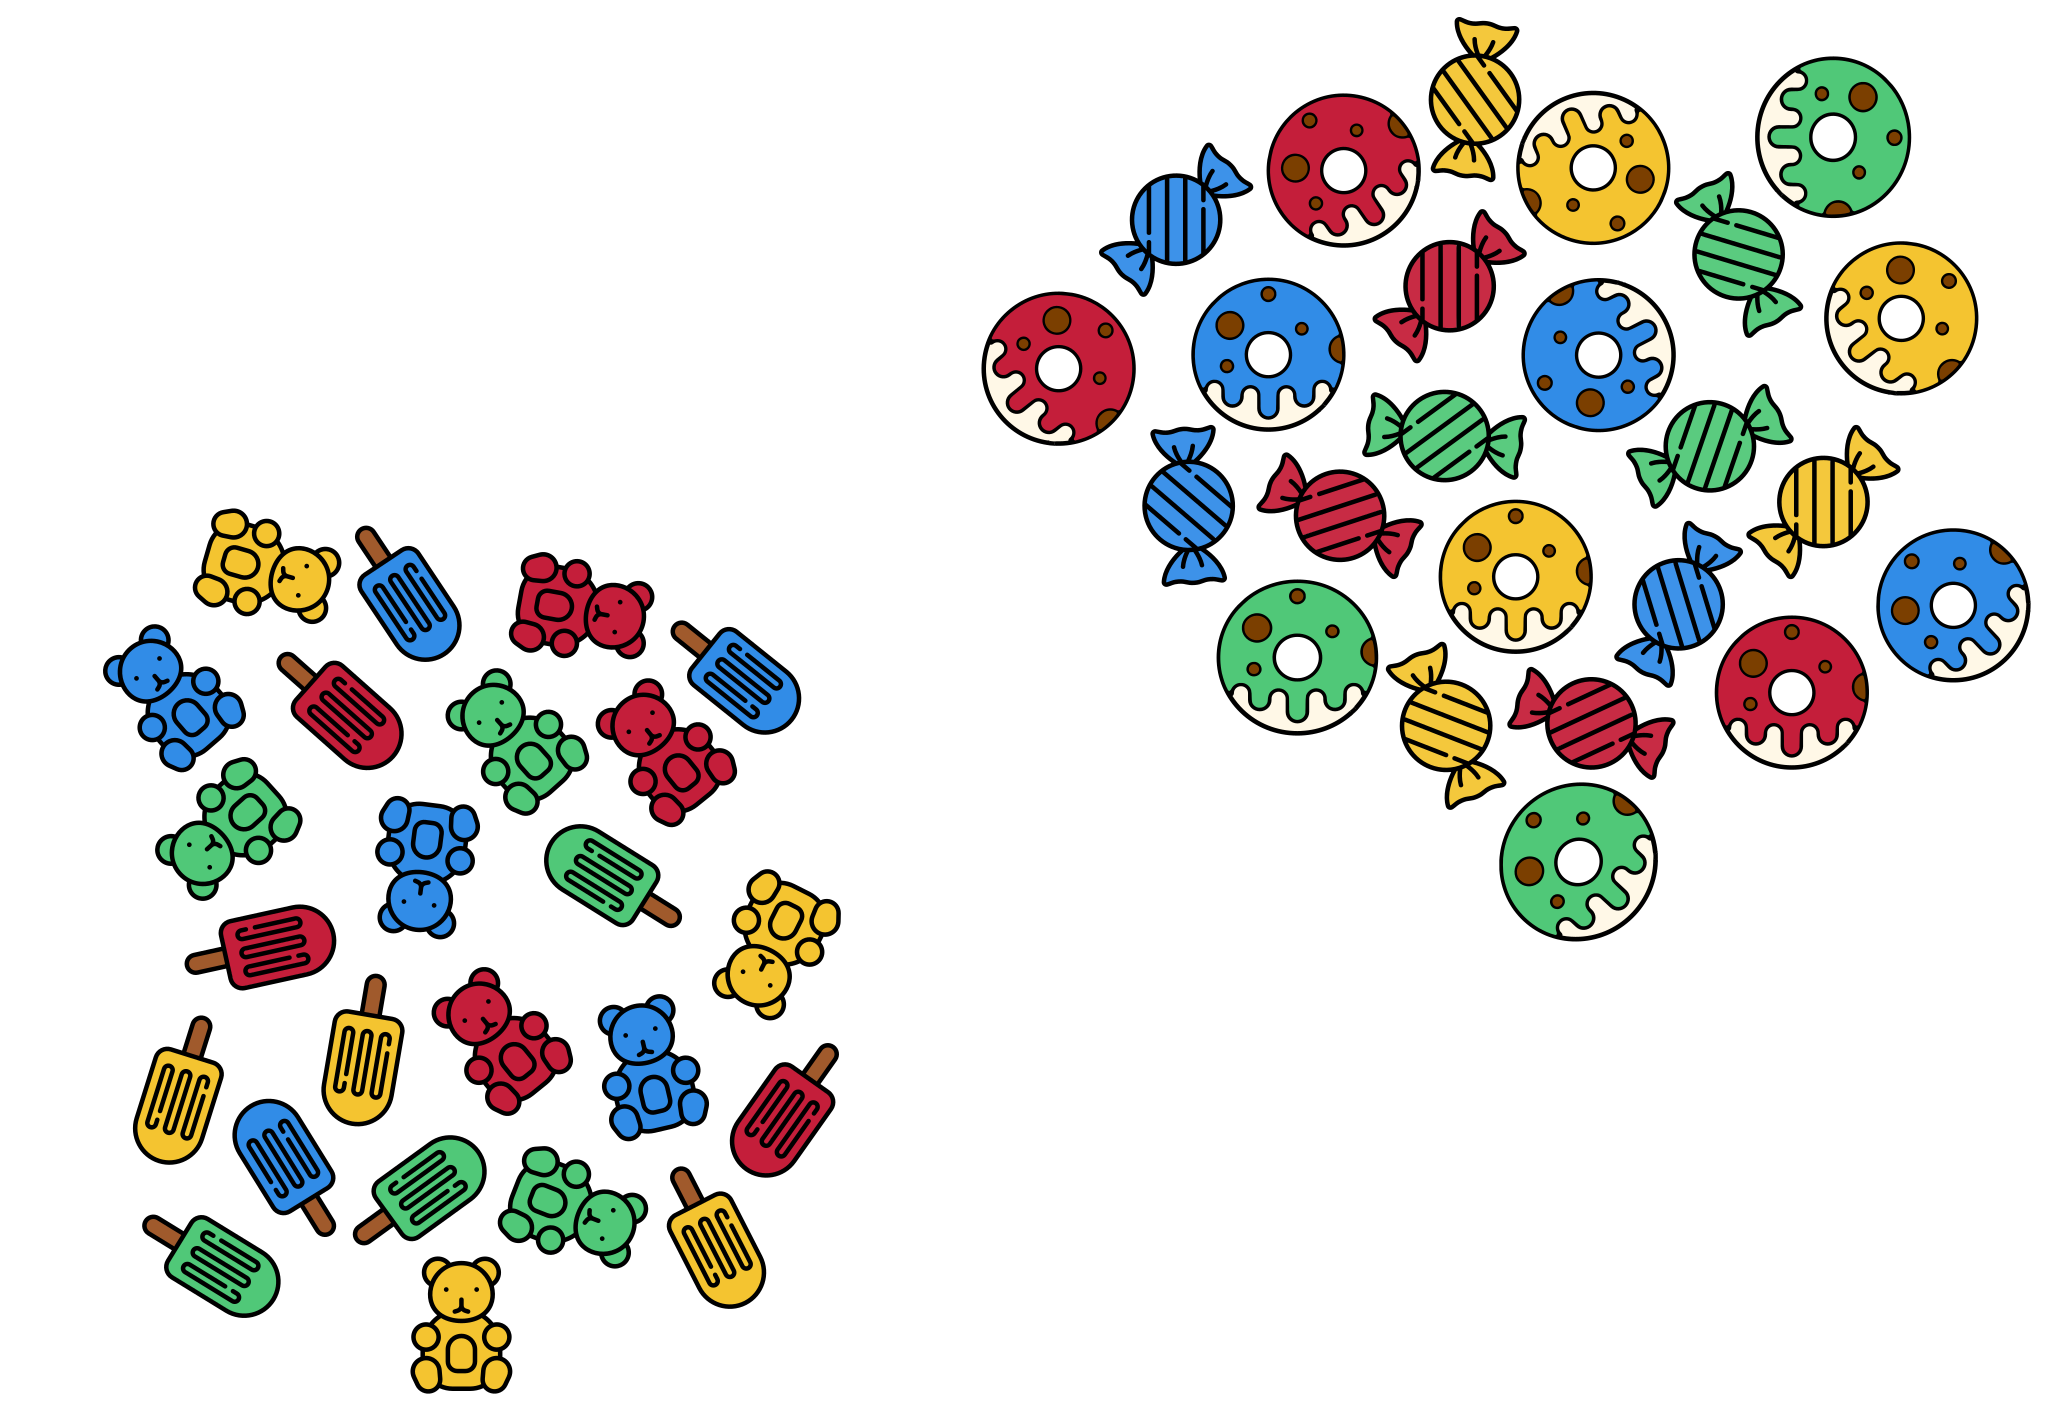
\includegraphics[width=0.75\linewidth]{Figures/Clustering_by_ingredients}
    \end{figure}
  \end{frame}

  \begin{frame}{A zoo of clustering methods}
    \begin{itemize}
      \item Hierarchical clustering~(agglomerative, divisive, \dots)
      \item \texttt{$k$-means}
      \item Density-based clustering~(\texttt{DBSCAN}, \texttt{DENCLUE})
    \end{itemize}
  \end{frame}


  \begin{frame}
    \begin{figure}
      \begin{tikzpicture}
        \tikzset{%
          every mark/.append style = {
            mark size = 0.35pt,
          }
        }
        %
        \pgfplotsset{%
          /pgfplots/scatter/use mapped color = {
            draw = mapped color,
            fill = mapped color,
          }
        }
        %
        \begin{groupplot}[%
          group style = {%
            group size     = 3 by 4,
            horizontal sep = 0pt,
            vertical sep   = 0pt,
          },
          %
          axis lines = none,
          clip mode  = individual,
          height     = 3.5cm,
          width      = 3.5cm,
        ]
          \nextgroupplot
            \addplot[%
              scatter,
              only marks,
              point meta=explicit
            ] table[meta index=2] {Data/AgglomerativeClustering_0.txt};
            \node at (rel axis cs:0.5,1.075) {\small Agglomerative};

          \nextgroupplot

            \addplot[%
              scatter,
              only marks,
              point meta=explicit
            ] table[meta index=2] {Data/MiniBatchKMeans_0.txt};
            \node at (rel axis cs:0.5,1.10) {\small\texttt{$k$-means}};

          \nextgroupplot

            \addplot[%
              scatter,
              only marks,
              point meta=explicit
            ] table[meta index=2] {Data/DBSCAN_0.txt};
            \node at (rel axis cs:0.5,1.10) {\small\texttt{DBSCAN}};

          \nextgroupplot
            \addplot[%
              scatter,
              only marks,
              point meta=explicit
            ] table[meta index=2] {Data/AgglomerativeClustering_1.txt};

          \nextgroupplot

            \addplot[%
              scatter,
              only marks,
              point meta=explicit
            ] table[meta index=2] {Data/MiniBatchKMeans_1.txt};

          \nextgroupplot

            \addplot[%
              scatter,
              only marks,
              point meta=explicit
            ] table[meta index=2] {Data/DBSCAN_1.txt};

          \nextgroupplot
            \addplot[%
              scatter,
              only marks,
              point meta=explicit
            ] table[meta index=2] {Data/AgglomerativeClustering_2.txt};

          \nextgroupplot

            \addplot[%
              scatter,
              only marks,
              point meta=explicit
            ] table[meta index=2] {Data/MiniBatchKMeans_2.txt};

          \nextgroupplot

            \addplot[%
              scatter,
              only marks,
              point meta=explicit
            ] table[meta index=2] {Data/DBSCAN_2.txt};

          \nextgroupplot
            \addplot[%
              scatter,
              only marks,
              point meta=explicit
            ] table[meta index=2] {Data/AgglomerativeClustering_5.txt};

          \nextgroupplot

            \addplot[%
              scatter,
              only marks,
              point meta=explicit
            ] table[meta index=2] {Data/MiniBatchKMeans_5.txt};

          \nextgroupplot

            \addplot[%
              scatter,
              only marks,
              point meta=explicit
            ] table[meta index=2] {Data/DBSCAN_5.txt};

        \end{groupplot}
      \end{tikzpicture}
    \end{figure}
  \end{frame}

  \begin{frame}{Similarity measures}
    \begin{center}
      \begin{tabular}{ll}
        \toprule
        \emph{Which metric should I use for}\dots? & \\
        \midrule
        Continuous data~({\small temperature, length, \dots}) & Euclidean distance, Mahalanobis distance\\
        Categorical data~({\small blood type, sex, \dots})    & Hamming distance\\
        Images                                                & Euclidean distance~(?)\\
        Graphs                                                & Weisfeiler--Lehman graph kernels\\
        Time series                                           & Dynamic time warping~(DTW)\\
        \bottomrule
      \end{tabular}
    \end{center}
  \end{frame}

  \begin{frame}{How to choose $k$?}
    \begin{itemize}
      \item \emph{$\beta$-CV}: ratio of mean intracluster distance to mean intercluster distance
      \item \emph{C index}: ratio of intracluster distances to sum of the largest distances between points
      \item \emph{Dunn index}: ratio of smallest distance between points in different clusters to largest diameter of a cluster
      \item \emph{Silhouette score}: ensures that clusters are \emph{cohesive} while also being \emph{separate}
    \end{itemize}
    %
    \vfill
    %
    All of these measures have their shortcomings, though, and can be
    ``tricked''. Ideally, ground truth information is available to
    verify a clustering.
  \end{frame}
\end{document}
